\subsection{Functional enrichment estimates for genes in corems}

We computed functional enrichment for genes organized into corems
using \tmsamp{DAVID} \cite{Dennis2003} and the
\tmsamp{DAVIDQuery} \cite{Day2010}
\tmsamp{R}-package. Enrichments for each corem are available on the
\href{http://egrin2.systemsbiology.net}{web site}.

\subsection{Conditional co-regulation of genes organized in corems}
\label{section:rsd}

We defined the conditions in which genes in a corem were co-regulated
as the set of experiments in which the genes of a corem are more
tightly co-expressed than one would expect at chance. We statistically
evaluated tight co-expression using relative standard deviation (RSD 
$=|\sigma/\mu|$) by resampling. We chose RSD (rather than, for example,
standard deviation, $\sigma$) to avoid over-weighting conditions in which the
mean relative expression is close to zero. The significance of an RSD
value for a given condition relative to each corem was estimated
by resampling: for a corem with $k$ gene members, and for each
condition, $c$, we computed at least 20,000 RSD values for $k$ randomly
sampled expression measurements in $c$, to determine the likelihood that the
observed co-expression has lower RSD than expected by chance ($p$-value
$< 0.01$). The resampling procedure resulted in condition sets for
corems that contained from 1.4\% to 85.5\% of the conditions in
\halo\ and 7.9\% to 66.6\% conditions in \eco\ (Figure \ref{fig:corem_stats}).

\subsection{Conditionality of GRE influence}

The upstream promoter regions of most genes contain multiple
\egrine-predicted GREs (\eg, \textit{carA} in Figure 2). A key insight
of our model is that not all of these sites are equally important for
controlling gene expression in all experimental conditions. We refer
to changes in the relative influence of GREs across conditions as
``conditional activity'' of GRE elements. Although, to be clear, we do
not imply that the transcriptional activity at a GRE is attributable
to the DNA sequence itself, but rather the TF that binds to that
sequence in particular environments. We leveraged the GREs discovered
in genes grouped into corems and the conditional co-expression of
those groups of genes to predict conditionally active GREs in \egrine.

To identify the active GREs for each corem we combined predictions
from (1) genome-wide motif scans (Section~\ref{section:scanning}
above) that predict the GRE locations in an expanded region around
each gene’s promoter in the corem using all of the ensemble
predictions (1,000 nt window: -875 nt upstream to 125 nt downstream),
and (2) the conditions discovered in biclusters that are most
representative of the corem (\ie, containing the largest fraction of
genes from the corem, top decile). GREs that occurred frequently
in these biclusters were considered putatively responsible for
co-regulating the set of genes in the condition-specific context of
the corem ($q$-value $\leq$ 0.05). Finally, we computed the average distances
of all GREs to the start codons of each gene in the list (collapsing
sites if they occurred within 25 nt of one another). The precise
locations of all GREs for the {\it H. salinarum} \textit{dpp} operon-related
corems (Figure 3) are listed in Table E8, while the locations of GREs
involved in conditional modulation of the PurR regulon (Figure 4) are
provided in Table E9.

We represented the active GREs upstream of a gene or within a corem as
a pie chart, showing the normalized frequency with which the GREs
computed above occurred in biclusters containing that gene. For
example, if GREs 1, 2, and 3 occurred in 25, 50, and 200 biclusters
containing gene $A$, the pie chart for gene $A$ would have sectors of area
0.09, 0.18, and 0.73 respectively. For corems, we computed the
normalized frequency of GREs for all genes of the corem. For example,
if GREs 1, 2, and 3 occurred in promoters of 10, 10, and 20 of the
genes of the corem, their areas would be 0.25, 0.25, and 0.5
respectively.

\begin{figure}[h!]
\centering
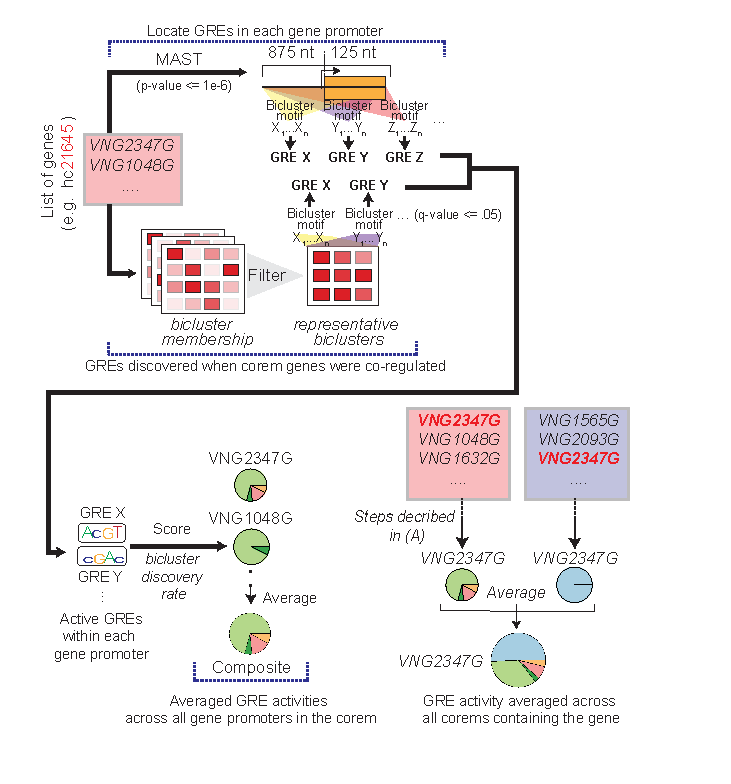
\includegraphics[width=0.7\linewidth]{figures/corem_gres.pdf}
\caption[Deciphering GREs responsible for regulating corems]{\textbf{Deciphering GREs responsible for regulating corems.} A GRE is implicated in regulation of a corem when it is both (1) located within an expanded region (-875nt to +125nt) around the translation start site of any gene in the corem; and (2) present in biclusters containing a large fraction of corem genes (top decile). Relative GRE influence is computed as the frequency with which each GRE was discovered in these representative biclusters (see Supplementary Methods for more details). Influence scores are illustrated as pie charts and reported for each gene individually (\eg, \textit{VNG2347G}); and as a composite by averaging across all genes in a corem. The width of each sector in the pie charts is proportional to the frequency of GRE discovery.}
\label{fig:corem_gres}
\end{figure}

\subsection{Detection of conditional operons}
\label{section:condop}
Condition-specific transcriptional isoforms of operons were predicted
through corem membership. If any of the genes in an operon were found
in a corem that did not contain all the other genes of the operon, we
predicted that the operon had conditional isoforms. Operon annotations
for both {\it H. salinarum} and {\it E. coli} were derived from
\tmsamp{MicrobesOnline} \cite{Alm2005,Price2005b}. All predicted conditional
operons, including the specific break sites and transcriptional
isoforms is available on the website. The full list of validated
predictions is provided in Table E7.

\subsection{Environmental ontology construction and usage}

We recorded a rich set of meta-data for all 1,495 experiments
conducted with {\it H. salinarum} and used for construction of the
\halo~ \egrine~model. The meta-data includes a detailed description
of each experiment, including, for example: media composition, genetic
background, concentration of perturbant, internal reference batch id,
person who conducted the experiment, etc. We used this
meta-information to classify experiments in an ontological framework,
where two experiments can share specific meta-descriptions (\eg,
$10^{-3}$ mol/L EDTA), or inherit more general relationships from the
ontological structure (\eg, chemical perturbation). We used OBO-edit
\cite{Day-Richter2007} to construct the ontology. The ontology contained 198
terms organized across three primary branches (environmental state,
experimental state, and genetic state). The ontology flat file is
available for download and meta-data annotations for every array in
the dataset are available \href{http://egrin2.systemsbiology.net}{online}.

\begin{figure}[h!]
\centering
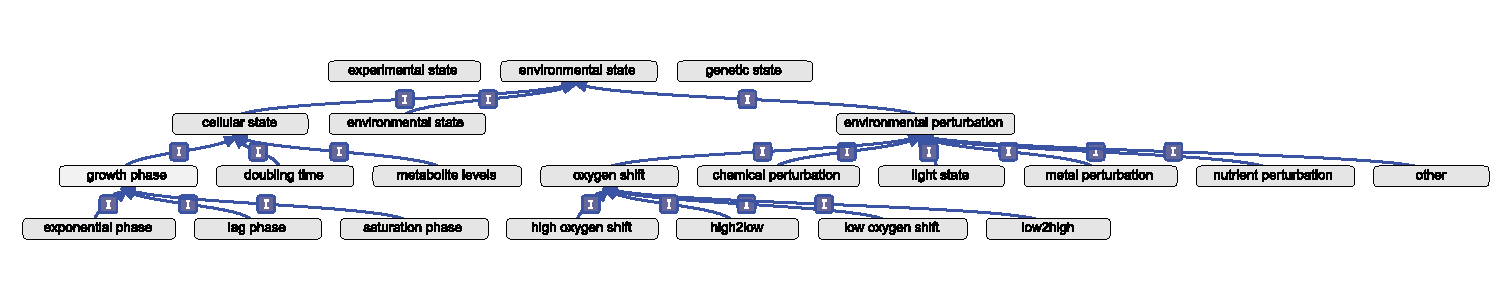
\includegraphics[width=0.95\linewidth]{figures/eo.pdf}
\caption[Environmental ontology hierarchically organizes relationships between experimental conditions from metadata collected across 1495 experiments in \textit{H. salinarum}]{{\bf Environmental ontology hierarchically organizes relationships between experimental conditions from metadata collected across 1495 experiments in \textit{H. salinarum}.} Subset of the environmental ontology constructed for \textit{H. salinarum} demonstrates many “is-a” (boxed ‘I’) relationships that organize similarities between descriptor terms descending from one of three root nodes (i.e., generic categorical descriptions). In this case a generic ontological term called `environmental state' gives rise to much more specific terms (e.g., exponential phase or high oxygen shift) that inherit (at the highest level) a relationship through their being related to the ‘environmental state’ of cells in the experiment. Each condition in the compendium is annotated with the most specific descriptors relevant to the experiment given metadata. The full environmental ontology is available for download from \href{http://egrin2.systemsbiology.net}{http://egrin2.systemsbiology.net}.}
\label{fig:eo}
\end{figure}

We used the ontology to classify enriched environmental features for
GREs and corems (Figures 3-4). For corems, we used the set of
conditions in which genes in the corem are significantly co-expressed
(see Section \ref{section:rsd} above) to compute term enrichment using the \tmsamp{ontoCAT}
\cite{Kurbatova2011}  \tmsamp{R}-package. Term enrichment was assessed
statistically and reported as $q$-values using the hypergeometric test
with Benjamini-Hochberg correction for multiple hypothesis testing.
